\documentclass[11pt]{article}
\usepackage[margin=1in]{geometry}
\usepackage[T1]{fontenc}
\usepackage{lmodern}
\usepackage{amsmath,amssymb}
\usepackage{booktabs}
\usepackage{graphicx}
\usepackage{xcolor}
\usepackage[hidelinks]{hyperref}
\usepackage[numbers,sort&compress]{natbib}
\usepackage{caption}
\captionsetup{font=small,labelfont=bf}

\title{Physics as a Checksum: Detecting the Harm, Not the Fault,\\in Detection-and-Tracking Pipelines}
\author{Jinhao Yang\\Xiamen University of Technology}
\date{}

\begin{document}
\maketitle

\begin{abstract}
Hardware faults such as bit flips from voltage underscaling, radiation or marginal silicon can silently corrupt the output of a neural network. In a perception pipeline the detector is rarely the end of the computation: its boxes feed a multi-object tracker, which already filters noisy detections. We ask how much of the fault problem the tracker solves by itself, and how to protect what is left without duplicating the network. In a campaign of 48{,}000 single bit flips across eight configurations (five detectors, two trackers, three datasets), the tracker fully masks 94.6--96.3\% of the faults that change the detector's output. We therefore monitor the consequences of faults rather than the faults themselves: a black-box monitor combines Kalman-innovation and frame-to-frame consistency statistics through Fisher's method, sets its threshold by split-conformal calibration, and re-executes the detector only on an alarm. On a sealed test split evaluated once under a frozen protocol, at one fault per inference, the monitor recovers 72--99\% of the HOTA loss for 2.6--9.1\% extra compute, while dual modular redundancy recovers 10--44\% for 140--187\%. A white-box activation-range monitor recovers 88--109\% but needs internal access and 19--22\% extra compute, because it reacts to every out-of-range activation, including the many that the tracker would have masked. Combined with range restriction, our monitor recovers 83--102\% for 1.6--6.7\%. A single-reduction checksum over all weights catches every persistent weight fault for 1.2--7.7\% of inference time. We also report where the method falls short: the false alarm guarantee breaks under within-sequence drift on MOT20 (3.65\% at a nominal 1\%), recovery is lowest on KITTI (72\%), and a sanitizer that looked effective on development data did not hold up on the sealed test.
\end{abstract}

\section{Introduction}

Silent data corruption is no longer a corner case. Fleet-scale studies report CPUs that compute wrong results without raising any error \citep{hochschild2021cores,dixit2021sdc}, and accelerators run at reduced voltage to save energy trade timing margins for occasional bit errors \citep{zhang2018thundervolt}. Neural networks are partly resilient, but a single flip in a high exponent bit can turn an activation into a huge value and change the network's output \citep{li2017understanding,reagen2018ares}.

Most fault-tolerance work for neural networks studies the network in isolation and asks whether its output changed. In deployed perception systems the network's output is an intermediate result. A detector produces boxes; a tracker associates them over time, keeps tracks alive through missed detections and ignores isolated spurious boxes. A fault that changes one frame's detections may therefore never change the tracks that the rest of the system consumes. If that is common, protecting every inference wastes effort on faults that do no harm, and the right question is not ``did a fault occur'' but ``did a fault cause harm''.

This paper makes four contributions.
\begin{enumerate}
\item \textbf{Measurement of tracker masking.} Across eight detector, tracker and dataset configurations, the tracker fully masks 94.6--96.3\% of the transient activation faults that change the detector output (Table~\ref{tab:masking}). Only 0.2--2.0\% of all injected faults leave a tracking error that outlives the faulty frame.
\item \textbf{A black-box monitor with a calibrated false alarm rate.} The monitor reads only the detector output and the tracker state. It tests each frame against the Kalman filter's predictions and against the previous frame, combines the statistics with Fisher's method, and sets the alarm threshold by split-conformal calibration on clean data, so that the false alarm rate, and therefore the re-execution cost on fault-free frames, is set in advance.
\item \textbf{Matched-fault comparison with standard defences.} Every policy sees the same fault sequence. Against no protection, range restriction \citep{chen2021ranger}, dual modular redundancy (DMR), a white-box activation-range monitor and an oracle, the monitor sits at the low-cost end of the cost and recovery trade-off (Fig.~\ref{fig:pareto}), and it composes with range restriction.
\item \textbf{A sealed evaluation.} All settings were frozen on development data and written to a protocol file before the test split was touched; the test split was evaluated once. We report the results that did not replicate as well as those that did.
\end{enumerate}
Persistent weight faults, which a per-frame output monitor sees only at their onset, are handled by a separate single-reduction checksum over all parameters.

\section{Related work}

\textbf{Fault injection and resilience of neural networks.} Fault injection studies \citep{li2017understanding,reagen2018ares,mahmoud2020pytorchfi} show that most single bit flips are masked inside the network, that exponent bits dominate the harmful cases, and that resilience depends on layer and data type. We use the same kind of injection but follow the error past the network into a tracker and measure harm with a tracking metric.

\textbf{Low-cost correction inside the network.} Range restriction (Ranger) clips activations to bounds profiled on clean data \citep{chen2021ranger}. Algorithm-based fault tolerance protects linear layers with checksums \citep{huang1984abft}. Both need access to the network's internals; range restriction also faces a trade-off between tight bounds, which change clean outputs, and wide bounds, which leave large errors in place. We evaluate it as a baseline and as a complement.

\textbf{Fault tolerance in perception and tracking.} VAP \citep{wan2024vap} assigns protection effort across an autonomous machine's software stack according to each component's robustness, using lightweight anomaly detection for the perception front end, so output-level temporal checking itself is not new. Milazzo et al.\ \citep{milazzo2025fault} study transient faults in deep multi-object tracking, find that activation clipping helps little, and correct faulty features using frame-to-frame feature similarity inside the network. Our monitor differs in three ways: it uses the tracker's own motion model rather than network features; it controls the false alarm rate with conformal calibration rather than a tuned threshold; and it is evaluated against matched-fault baselines, including a white-box monitor, on a sealed test split.

\textbf{Conformal prediction.} Split-conformal calibration gives finite-sample, distribution-free control of the rate at which an exchangeable clean sample exceeds a threshold \citep{vovk2005algorithmic,angelopoulos2021gentle}. Adaptive conformal inference adjusts the level online when the data drift \citep{gibbs2021aci}. We use both and test whether the guarantee survives the move from calibration to test data.

\section{Setting and fault model}

\textbf{Pipeline.} A detector (YOLOv8n/s/m, YOLO11s \citep{ultralytics} or RT-DETR-L \citep{zhao2024rtdetr}) runs in FP16 on every frame; its boxes feed ByteTrack \citep{zhang2022bytetrack} or SORT \citep{bewley2016sort}. We use MOT17 \citep{milan2016mot16}, MOT20 \citep{dendorfer2020mot20} and KITTI tracking (cars) \citep{geiger2012kitti}, and score tracking with HOTA \citep{luiten2021hota}. The eight configurations vary one factor at a time around MOT17 with YOLOv8s and ByteTrack.

\textbf{Splits.} Each sequence is split in time: the first 25\% (q1) is used only for clean statistics, the next 25\% (q2) for fault campaigns and design decisions, and the last 50\% (test) is sealed.

\textbf{Faults.} A transient fault flips one bit of one FP16 element in the output of one convolution or linear layer during one inference. The site is drawn uniformly over elements, with the layer chosen in proportion to its output size. The campaign uses all 16 bits; the end-to-end runs use the sign and exponent bits (the six high bits), where harmful faults concentrate, and Table~\ref{tab:allbit} repeats them with all 16 bits. A persistent fault flips one bit of one weight and stays until it is repaired. At fault rate $r$, each inference call, including re-executions, is hit with probability $r$; $r=1$ means every call is faulty.

\textbf{Harm.} Each fault is replayed through the tracker over a 30-frame window and compared with the fault-free run. The tracker \emph{masks} it if the tracks are identical over the whole window. It \emph{propagates} if the tracking error outlives the faulty frame (a track is lost, added or switched on later frames) or causes an identity switch. Its \emph{damage} is the number of false negatives, false positives and identity switches it causes over the window, measured against the fault-free tracks.

\section{Method}

\subsection{Frame statistics}
For each frame the monitor computes, from the detector output, the previous frame's output and the tracker state before the update:
\begin{itemize}
\item \emph{Kalman innovation:} for each established track matched to a confident box, the normalized innovation squared $y^\top S^{-1} y$ of the box against the track's predicted state \citep{barshalom2001}; the statistic is the maximum over matches, with a Bonferroni correction for the number of matches.
\item \emph{Unpredicted births:} confident boxes that overlap no predicted track.
\item \emph{Unexplained deaths:} established, fully visible tracks with no box nearby, counted once against all boxes and once against confident boxes only.
\item \emph{Frame-to-frame changes:} confident boxes with no counterpart in the previous frame, previous boxes with no counterpart now, and the change in the number of confident boxes.
\end{itemize}

\subsection{Calibrated combination}
Each statistic is turned into an empirical tail p-value against its distribution on clean q1 frames, and the p-values are combined with Fisher's method \citep{fisher1925}, $s = -2\sum_i \log p_i$. Fisher's statistic is used here as a score, not as a test with independent inputs: its threshold is set empirically. Following split-conformal calibration, the threshold at level $\alpha$ is the $\lceil(1-\alpha)(n+1)\rceil$-th smallest score on $n$ clean q2 frames that were not used to build the p-value tables. If clean test frames are exchangeable with clean q2 frames, the false alarm rate is at most $\alpha$; we test that assumption rather than assume it.

\subsection{Re-execution}
On an alarm the detector runs again on the same frame and the output with the lower score is passed to the tracker. A re-execution can itself be faulty; an oracle that knows the fault-free output and re-runs until it is reached gives an upper bound. For drift we also evaluate adaptive conformal inference \citep{gibbs2021aci} per camera stream with step $\gamma=0.005$, using the re-run as feedback: if the re-executed output equals the original, the alarm was false.

\subsection{Weights}
A persistent weight fault corrupts every later frame, so a per-frame output monitor sees it only at its onset. We move all floating-point parameters and buffers into one contiguous buffer per data type and compute the integer sum of their raw FP16 words in one reduction. Any single bit flip changes this sum, so the check has no false alarms and no misses for single flips.

\section{Experimental protocol}

All settings below were fixed on q1 and q2 and written to a protocol file before the test split was used: the combined monitor, split-conformal calibration (tables from q1, threshold from q2), $\alpha=1\%$ (and $0.1\%$), $\gamma=0.005$, 6000 transient faults per configuration with a fixed campaign seed, and end-to-end runs at $r\in\{0.1,0.3,1\}$ with three seeds. The baselines in Section~\ref{sec:baselines} were frozen the same way before their test runs. The evaluation script refuses to run if the protocol file changes. All policies at a given rate and seed see the same faults (common random numbers): the fault at each call depends only on the seed, rate, sequence, frame and attempt. False alarm intervals use a moving-block bootstrap \citep{kunsch1989jackknife} with blocks of 60 frames; detection rates use Wilson intervals. Timings are from one laptop GPU (RTX 3070 Ti) with faults emulated through framework hooks.

\section{Results}

\subsection{The tracker masks most output corruptions}
Table~\ref{tab:masking} shows the sealed campaign. Between 22\% (KITTI) and 59\% (MOT20) of single bit flips change the detector output, but for 94.6--96.3\% of those changes the tracks stay identical to the fault-free run over the whole 30-frame window. Only 14 to 117 of 6000 faults propagate. A defence that reacts to every changed output therefore spends most of its effort on harmless faults.

\begin{table}[t]
\centering\small
\caption{Tracker masking on the sealed test split (6000 transient single bit flips per configuration, all 16 bits).}
\label{tab:masking}
\resizebox{\linewidth}{!}{\begin{tabular}{lrrrr}
\toprule
configuration & detector output changed & fully masked by tracker & tracking changed & propagated \\
\midrule
MOT17 $\cdot$ YOLOv8n & 43.7\% & 96.3\% & 96 & 40 \\
MOT17 $\cdot$ YOLOv8s & 46.3\% & 96.0\% & 112 & 53 \\
MOT17 $\cdot$ YOLOv8m & 50.7\% & 96.0\% & 123 & 60 \\
MOT17 $\cdot$ YOLO11s & 51.5\% & 96.2\% & 116 & 60 \\
MOT17 $\cdot$ RT-DETR-L & 50.7\% & 95.1\% & 148 & 91 \\
MOT17 $\cdot$ YOLOv8s $\cdot$ SORT & 46.3\% & 95.9\% & 115 & 14 \\
MOT20 $\cdot$ YOLOv8s & 59.1\% & 96.3\% & 132 & 117 \\
KITTI $\cdot$ YOLOv8s & 21.9\% & 94.6\% & 71 & 23 \\
\bottomrule
\end{tabular}
}
\end{table}

\subsection{False alarms and detection}
Table~\ref{tab:monitor} and Fig.~\ref{fig:far} report the monitor at $\alpha=1\%$. On seven configurations the clean false alarm rate on the test split is 0.51--1.25\%, consistent with the nominal level. On MOT20 it is 3.65\% (95\% CI 2.24--5.32\%): crowded scenes change between the first and second half of each sequence, so test frames are not exchangeable with calibration frames. Adaptive calibration brings MOT20 to 0.77\% and all configurations to 0.47--0.94\%, at a cost discussed in Section~\ref{sec:limits}. The monitor detects 69--94\% of propagated faults, and the faults it detects carry 75--99\% of their damage, because the faults it misses are mostly small.

\begin{table}[t]
\centering\small
\caption{Monitor on the sealed test split at nominal $\alpha=1\%$. FAR: false alarms on clean test frames. Damage caught: share of the damage of propagated faults that comes from faults the monitor flags.}
\label{tab:monitor}
\resizebox{\linewidth}{!}{\begin{tabular}{lrrrrrr}
\toprule
configuration & FAR fixed [95\% CI] & FAR adaptive & propagated faults & TPR [95\% CI] & damage caught & FAR white-box \\
\midrule
MOT17 $\cdot$ YOLOv8n & 0.98\% [0.43, 1.59] & 0.94\% & 40 & 87.5\% [73.9, 94.5] & 95.8\% & 0.23\% \\
MOT17 $\cdot$ YOLOv8s & 0.51\% [0.15, 0.96] & 0.63\% & 53 & 94.3\% [84.6, 98.1] & 99.3\% & 2.11\% \\
MOT17 $\cdot$ YOLOv8m & 0.55\% [0.20, 0.97] & 0.47\% & 60 & 81.7\% [70.1, 89.4] & 96.4\% & 2.15\% \\
MOT17 $\cdot$ YOLO11s & 1.25\% [0.66, 1.95] & 0.70\% & 60 & 90.0\% [79.9, 95.3] & 96.4\% & 3.21\% \\
MOT17 $\cdot$ RT-DETR-L & 0.78\% [0.36, 1.29] & 0.55\% & 91 & 69.2\% [59.1, 77.8] & 88.6\% & 0.04\% \\
MOT17 $\cdot$ YOLOv8s $\cdot$ SORT & 0.74\% [0.32, 1.24] & 0.59\% & 14 & 92.9\% [68.5, 98.7] & 96.2\% & 2.11\% \\
MOT20 $\cdot$ YOLOv8s & 3.65\% [2.24, 5.32] & 0.77\% & 117 & 91.5\% [85.0, 95.3] & 99.4\% & 0.29\% \\
KITTI $\cdot$ YOLOv8s & 0.51\% [0.24, 0.83] & 0.51\% & 23 & 82.6\% [62.9, 93.0] & 75.3\% & 1.81\% \\
\bottomrule
\end{tabular}
}
\end{table}

\begin{figure}[t]
\centering
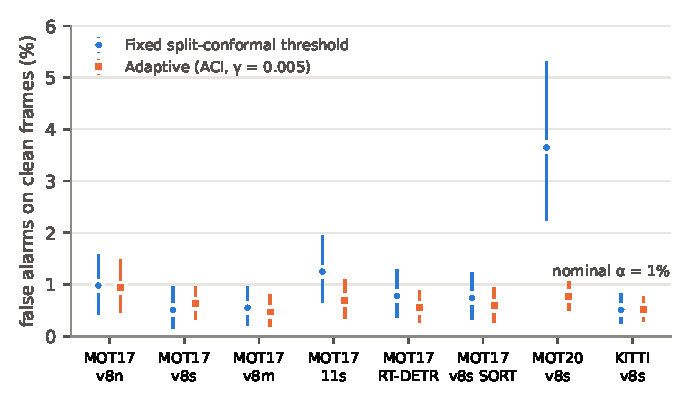
\includegraphics[width=0.75\linewidth]{fig_far.pdf}
\caption{Clean false alarm rate on the sealed test split with 95\% block-bootstrap intervals. The fixed split-conformal threshold holds on seven of eight configurations; on MOT20 within-sequence drift breaks exchangeability. Adaptive calibration restores the level.}
\label{fig:far}
\end{figure}

\subsection{End-to-end protection and baselines}\label{sec:baselines}
Fig.~\ref{fig:pareto} and Table~\ref{tab:e2e} compare policies at one fault per inference. Without protection, HOTA drops by 1.35--3.32 points.
\begin{itemize}
\item \textbf{DMR} recovers only 10--44\% of the loss for 140--187\% extra compute. At high fault rates both runs are often faulty, and every harmless difference triggers more work.
\item \textbf{Range restriction} with bounds wide enough to leave all sampled clean outputs unchanged (0 of 533--895 frames) recovers 13--36\%: an exponent flip clipped to a wide bound is still a large error.
\item \textbf{The white-box range monitor}, calibrated the same way as ours, recovers 88--109\% but re-executes 19--22\% of frames, because it flags any out-of-range activation, harmful or not.
\item \textbf{Our monitor} recovers 72--99\% for 2.6--9.1\%, and \textbf{with range restriction} 83--102\% for 1.6--6.7\%. The two compose: clipping removes part of the damage at almost no cost, and the monitor catches what remains with fewer alarms.
\end{itemize}
The oracle shows the ceiling: 93--101\% for 44--183\%. With the flipped bit uniform over all 16 bits (Table~\ref{tab:allbit}), losses are smaller and the ordering is unchanged: our monitor recovers 73--102\% for 1.5--5.5\%, DMR 1--69\% for 134--182\%.

\begin{figure}[t]
\centering
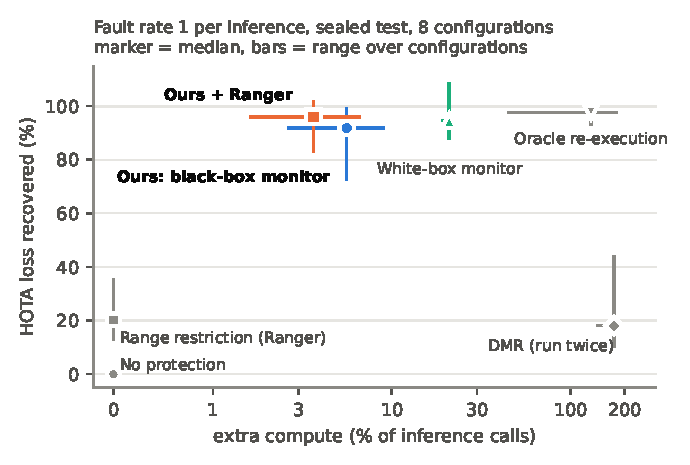
\includegraphics[width=0.75\linewidth]{fig_pareto.pdf}
\caption{HOTA loss recovered against extra compute at one fault per inference (sign and exponent bits), sealed test split. Markers are medians over the eight configurations; bars span their range.}
\label{fig:pareto}
\end{figure}

\begin{table}[t]
\centering\small
\caption{End to end at one fault per inference: HOTA loss recovered / extra inference calls. Three seeds, identical faults for every policy.}
\label{tab:e2e}
\resizebox{\linewidth}{!}{\begin{tabular}{lrrrrrrr}
\toprule
configuration & dHOTA unprotected & Ranger & DMR & oracle & white-box & ours & ours + Ranger \\
\midrule
MOT17 $\cdot$ YOLOv8n & -1.55 & 18\% / 0.0\% & 17\% / 173.0\% & 97\% / 105.3\% & 95\% / 20.7\% & 99\% / 6.0\% & 102\% / 3.5\% \\
MOT17 $\cdot$ YOLOv8s & -1.60 & 22\% / 0.0\% & 14\% / 173.6\% & 99\% / 121.4\% & 99\% / 21.6\% & 94\% / 5.3\% & 96\% / 3.3\% \\
MOT17 $\cdot$ YOLOv8m & -2.99 & 13\% / 0.0\% & 18\% / 175.6\% & 93\% / 147.1\% & 95\% / 20.8\% & 88\% / 5.6\% & 95\% / 3.7\% \\
MOT17 $\cdot$ YOLO11s & -3.25 & 36\% / 0.0\% & 21\% / 178.6\% & 97\% / 138.3\% & 95\% / 22.0\% & 95\% / 6.2\% & 98\% / 4.0\% \\
MOT17 $\cdot$ RT-DETR-L & -1.58 & 16\% / 0.0\% & 18\% / 182.8\% & 99\% / 139.7\% & 109\% / 18.9\% & 92\% / 5.4\% & 97\% / 3.8\% \\
MOT17 $\cdot$ YOLOv8s $\cdot$ SORT & -1.35 & 26\% / 0.0\% & 26\% / 173.6\% & 99\% / 121.4\% & 91\% / 21.6\% & 89\% / 5.6\% & 96\% / 3.6\% \\
MOT20 $\cdot$ YOLOv8s & -3.32 & 16\% / 0.0\% & 10\% / 186.7\% & 93\% / 182.9\% & 88\% / 20.5\% & 92\% / 9.1\% & 96\% / 6.7\% \\
KITTI $\cdot$ YOLOv8s & -1.69 & 34\% / 0.0\% & 44\% / 139.8\% & 101\% / 44.4\% & 92\% / 21.1\% & 72\% / 2.6\% & 83\% / 1.6\% \\
\bottomrule
\end{tabular}
}
\end{table}

\begin{figure}[t]
\centering
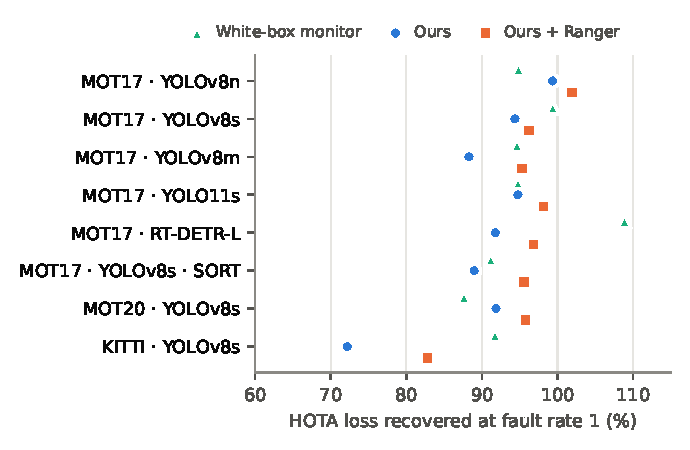
\includegraphics[width=0.75\linewidth]{fig_recovery.pdf}
\caption{Recovery per configuration at one fault per inference. The white-box monitor (19--22\% extra compute) recovers more on YOLOv8s, KITTI and RT-DETR; our monitor with range restriction (1.6--6.7\%) matches or exceeds it on the other five.}
\label{fig:recovery}
\end{figure}

\subsection{Weight faults}
Table~\ref{tab:checksum} gives the cost of the all-parameter checksum. One reduction over 3.2--32.1 million FP16 words takes 0.15--1.39\,ms, 1.2--7.7\% of an inference, and caught all 200 random single bit flips on every model. Computing one checksum per layer instead costs 3.9--10.8\,ms because it launches one small reduction per layer. In a replay of corrupting weight faults on YOLOv8s, checking every frame stopped all of them from reaching the tracks; checking every second frame let 27\% through.

\begin{table}[t]
\centering\small
\caption{All-parameter weight checksum per frame.}
\label{tab:checksum}
\resizebox{0.85\linewidth}{!}{\begin{tabular}{lrrrrr}
\toprule
detector & parameters & checksum & inference & overhead & random flips caught \\
\midrule
YOLOv8n & 3.2 M & 0.15 ms & 13.0 ms & 1.16\% & 200/200 \\
YOLOv8s & 11.2 M & 0.50 ms & 13.2 ms & 3.75\% & 200/200 \\
YOLOv8m & 25.9 M & 1.13 ms & 14.7 ms & 7.70\% & 200/200 \\
YOLO11s & 9.4 M & 0.42 ms & 17.3 ms & 2.43\% & 200/200 \\
RT-DETR-L & 32.1 M & 1.39 ms & 29.7 ms & 4.70\% & 200/200 \\
\bottomrule
\end{tabular}
}
\end{table}

\subsection{Development versus sealed results}
Table~\ref{tab:devtest} places the development numbers next to the sealed ones. Detection and recovery replicate within a few points; the MOT20 false alarm rate does not.

\section{Limitations}\label{sec:limits}

\textbf{Drift breaks the guarantee.} Split-conformal control assumes exchangeable clean frames. MOT20's crowd density changes within sequences, and the fixed threshold gave 3.65\% false alarms at a nominal 1\%. Adaptive calibration restores the level but lowers MOT20 detection of propagated faults from 91.5\% to 72.6\%. The white-box monitor also drifts (0.04--3.21\% at a nominal 1\%).

\textbf{Black-box observability.} On RT-DETR the monitor detects only 69\% of propagated faults. Many of the misses add a duplicate of a real object with a score just above the tracker's threshold, a change that clean frames also produce. A statistic cannot separate them without false alarms. On KITTI the monitor recovers 72\% of the loss, the lowest of all configurations.

\textbf{A development result that did not replicate.} On development data, class-agnostic NMS before the tracker seemed to make RT-DETR's duplicate-box faults harmless. On the sealed test it raised clean HOTA (40.74 to 41.00) by removing duplicates in fault-free frames, but did not reduce the damage of the faults the monitor misses. We therefore report it as an accuracy fix for NMS-free detectors, not as a fault defence.

\textbf{Measurement.} Faults are emulated with framework hooks on a laptop GPU, not injected in hardware or measured on an embedded accelerator; extra compute is counted in inference calls, and the cost of clipping itself is not counted. We do not yet translate compute into energy at reduced voltage.

\section{Conclusion}

In a detection-and-tracking pipeline, most corrupted detector outputs never reach the tracks. Monitoring the consequences of faults, with a threshold calibrated on clean data, recovers most of the tracking loss for a few percent of extra compute, an order of magnitude less than duplication or a white-box monitor, and it composes with range restriction. The sealed evaluation also shows where the approach needs more work: calibration under drift, and faults that look like ordinary detector noise.

\appendix
\section{Additional tables}

\begin{table}[h]
\centering\small
\caption{Bit model 'all' (flipped bit uniform over 16 bits), one fault per inference: HOTA loss recovered / extra compute.}
\label{tab:allbit}
\resizebox{0.85\linewidth}{!}{\begin{tabular}{lrrrr}
\toprule
configuration & dHOTA unprotected & DMR & oracle & ours \\
\midrule
MOT17 $\cdot$ YOLOv8n & -0.82 & 62\% / 165.8\% & 101\% / 84.4\% & 96\% / 2.9\% \\
MOT17 $\cdot$ YOLOv8s & -1.03 & 28\% / 168.1\% & 100\% / 95.4\% & 99\% / 2.6\% \\
MOT17 $\cdot$ YOLOv8m & -1.51 & 21\% / 170.8\% & 101\% / 116.3\% & 97\% / 2.4\% \\
MOT17 $\cdot$ YOLO11s & -1.13 & 34\% / 174.1\% & 100\% / 113.5\% & 93\% / 3.1\% \\
MOT17 $\cdot$ RT-DETR-L & -0.59 & 36\% / 176.6\% & 100\% / 102.9\% & 102\% / 2.7\% \\
MOT17 $\cdot$ YOLOv8s $\cdot$ SORT & -0.76 & 51\% / 168.1\% & 100\% / 95.4\% & 96\% / 2.8\% \\
MOT20 $\cdot$ YOLOv8s & -1.65 & 1\% / 181.5\% & 94\% / 141.5\% & 98\% / 5.5\% \\
KITTI $\cdot$ YOLOv8s & -0.95 & 69\% / 134.3\% & 100\% / 34.8\% & 73\% / 1.5\% \\
\bottomrule
\end{tabular}
}
\end{table}

\begin{table}[h]
\centering\small
\caption{Development (q2) versus sealed test, combined monitor at $\alpha=1\%$. The development false alarm rate is in-sample for the threshold by construction.}
\label{tab:devtest}
\resizebox{\linewidth}{!}{\begin{tabular}{lrrrrrr}
\toprule
configuration & FAR dev & FAR test & TPR dev & TPR test & recovered dev & recovered test \\
\midrule
MOT17 $\cdot$ YOLOv8n & 0.90\% & 0.98\% & 92.0\% & 87.5\% & 91\% & 99\% \\
MOT17 $\cdot$ YOLOv8s & 0.90\% & 0.51\% & 96.0\% & 94.3\% & 92\% & 94\% \\
MOT17 $\cdot$ YOLOv8m & 0.90\% & 0.55\% & 83.5\% & 81.7\% & 89\% & 88\% \\
MOT17 $\cdot$ YOLO11s & 0.90\% & 1.25\% & 88.7\% & 90.0\% & 81\% & 95\% \\
MOT17 $\cdot$ RT-DETR-L & 0.90\% & 0.78\% & 61.4\% & 69.2\% & 90\% & 92\% \\
MOT17 $\cdot$ YOLOv8s $\cdot$ SORT & 0.90\% & 0.74\% & 95.0\% & 92.9\% & 88\% & 89\% \\
MOT20 $\cdot$ YOLOv8s & 0.92\% & 3.65\% & 95.3\% & 91.5\% & 94\% & 92\% \\
KITTI $\cdot$ YOLOv8s & 0.89\% & 0.51\% & 80.0\% & 82.6\% & 72\% & 72\% \\
\bottomrule
\end{tabular}
}
\end{table}

\bibliographystyle{plainnat}
\bibliography{refs}
\end{document}
